\section*{Avant Propos}

Afin d'analyser et classifier des images 2D ou imageries 3D, il est primordial d'être capable d'extraire de ces dernières un ensemble d'informations ou "\textit{features}" qui décrivent au mieux et nous renseigne sur la nature de celle-ci.\\
On pourrait citer par exemple des critères comme la taille de la boite englobante (en anglais : \textit{bounding box}), ou encore le volume de la forme pour une pièce mécanique en 3D, en passant par la surface de cette dernière. Le critères isopérimétrique (mesure de compacité) est un excellent exemple de facteur classifiant. Il permet de discriminer, avec une bonne précision, différentes pièces mécaniques à partir de modèle 3D [M. Bruneau et al]~\cite{Bruneau2014}.

Dans le cadre de ce stage, nous nous focaliserons sur :\\
\begin{itemize}
	\item	L'accent sera porté sur une analyse d'\textbf{images en 2D}.\\
	\item	Nous cherchons à rétro-concevoir de grands ensembles mécaniques, une attention à la gestion de \textbf{grands volumes de données} doit être apportée durant tout le déroulement du projet.\\
	\item	Mettre en place une \textbf{méthode d'extraction} de descripteurs d'un fichier image (en anglais : \textit{Feature Extractor}).\\
	\item	Cette \textbf{méthode} d'extraction doit être \textbf{automatisable}. Il n'est pas envisageable, dans le cadre de notre étude, de venir renseigner à la main chacun de ces descripteurs.	
\end{itemize}
\vspace{3mm}
  

\section{Les Shock Graphs}

\subsection{État de l'art et méthodes d'extraction de descripteurs.}

Suite à trois semaines d'analyse de la littérature scientifique, il en est ressorti plusieurs méthodes qui pourraient satisfaire nos besoins. La plupart de ces méthodes sont directement dérivées du domaine de la \textbf{Vision par Ordinateur}.

J'ai testé plusieurs méthodes basées sur différentes approches du problèmes :
\begin{itemize}
	\item Filtre de Canny
	\item Algorithme SURF
	\item Réseaux de Convolutions
	\item Shock Graphs
	\item \ldots
\end{itemize}
\vspace{3mm}

\begin{figure}[H]
    \centering
    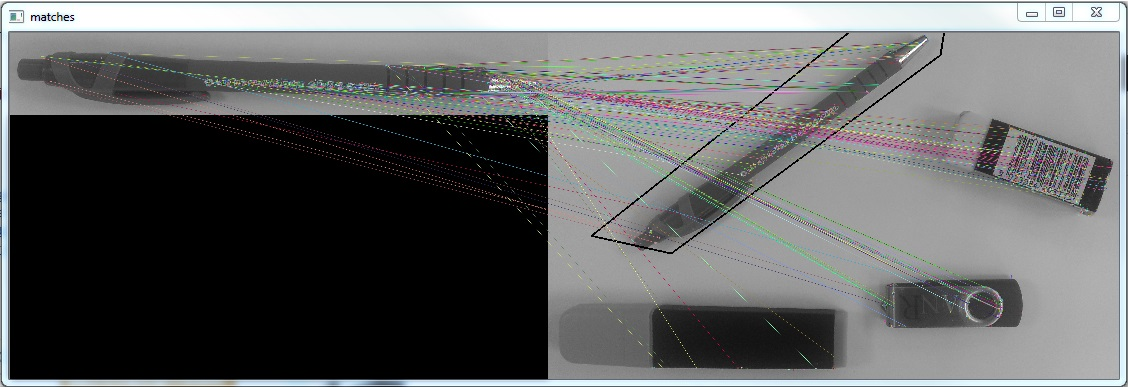
\includegraphics[height=5.5cm]{CannySurfClean.jpg}
	\caption{Output d'un test avec l'algorithme SURF, cible totalement visible} 
\end{figure}
\vspace{-6mm}

\begin{figure}[H]
    \centering
    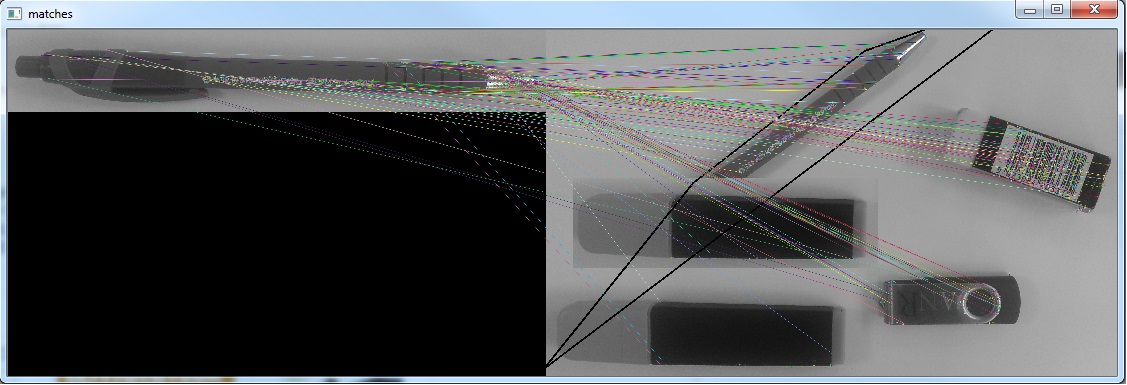
\includegraphics[height=5.5cm]{CannySurfPartiallyMasked.jpg}
	\caption{Output d'un test avec l'algorithme SURF, cible partiellement visible}\label{image.CannySurfPartiallyMasked} 
\end{figure}
\vspace{-6mm}

Il apparait que l'algorithme SURF manque de précision et vient \textit{accrocher} tous les objets de la scène. D'avantages d'investigations ont mis en évidence que l'algorithme étant basé sur la détection de points d'intérêt n'est pas capable d'apprendre une forme mais uniquement les détails d'un objet spécifique. Raisons qui font de l'algorithme SURF un \textbf{mauvais candidat} pour notre étude.

\clearpage
\subsection{Tests préliminaires sur le fonctionnement des Shock Graphs}

Suite à mes recherches bibliographiques, j'ai pu mettre en évidence les travaux sur les Shock Graphs. Ce sont des graphs qui décrivent une forme binaire 2D (Blanche ou Noire, pas de gris) par le biais d'un \textit{squelette} ou \textit{axe médian de Blum}. Leur fonctionnement et leur utilisation est décrite par [K. Siddiqi et al]~\cite{Siddiqi1999}. Un démonstrateur scientifique et une méthode de comparaison de ces graphs a été mise au point par [D. Macrini et al]~\cite{Macrini2002} dans le cadre de son mémoire de master.

À partir de ces travaux, j'ai pu mettre sur pied assez rapidement un test mettant en évidence la pertinence de la méthode relative à notre usage. Et je dois bien admettre avoir été bluffé par la précision de cette méthode. Sentiment qui semble avoir partagé autour de moi.

J'ai créé donc pour le test un jeu de données d'apprentissage et un jeu de test. Chacun contenant un ensemble de vues des pièces mécaniques suivantes:
\begin{itemize}
	\item 	Piston
	\item	Bielle
	\item	Assemblage Piston/Bielle
	\item	Roue dentée
\end{itemize}
\vspace{5mm}

\begin{figure}[H]
    \centering
    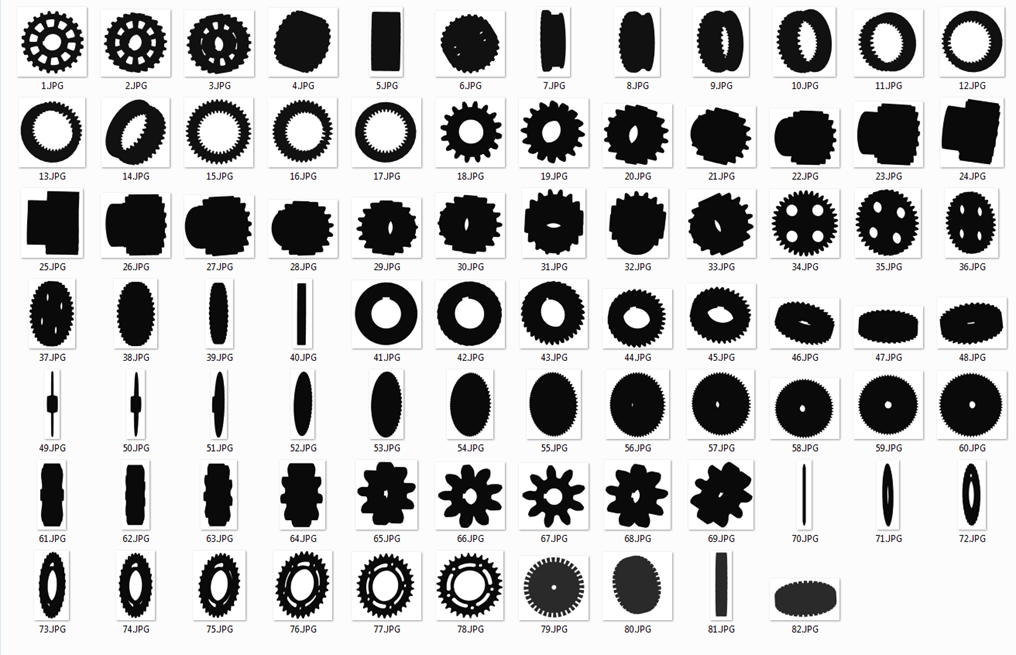
\includegraphics[height=7cm]{datasetShock.png}
	\caption{Exemple de base de connaissances sur les roues dentées, en vue du test des Shock Graphs}\label{image.ShockGearDataset} 
\end{figure}
\vspace{-4mm}

\begin{figure}[H]
    \centering
    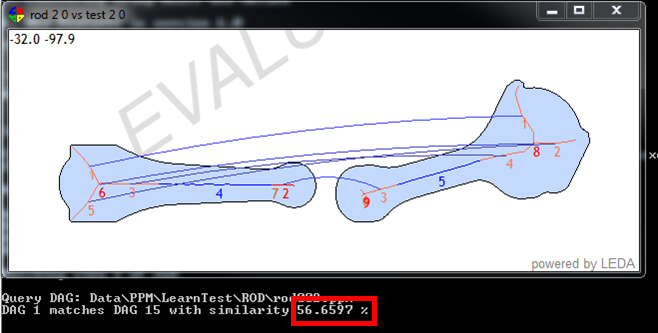
\includegraphics[height=5.5cm]{ShockTest1.png}
	\caption{Output d'un test utilisant les Shock Graphs, \textbf{56.6597\% de match}.}\label{image.ShockTest1} 
\end{figure}


\clearpage

\subsection{Principe de fonctionnement des Shock Graphs.}

Lotus Notes (solution logicielle développée par \textbf{IBM}) et Cordys Process Factory (solution Cloud développée \textbf{Open~Text}) ont un objectif commun : proposer une réponse au  besoin de ``\textit{Business Processing}" au sein d'une entreprise.

Cependant elles diffèrent sur l'architecture (serveurs et réseau) nécessaire à son fonctionnement :

\begin{itemize}
		\item Lotus Notes se base sur une architecture type logiciel Client / logiciel Serveur, les serveurs sont inter-connectés entre eux et ``\textit{répliquent}" certaines de leur données à intervalle de temps régulier. Ce fonctionnement est coûteux , il demande une infrastructure imposante ainsi qu'une administration au jour le jour. \\
		Plus gênant, comme il est difficile d'avoir une vue d'ensemble du système actuel, la quantité d'application dupliquée ne cesse d'augmenter, ce qui induit des coûts de fonctionnement de plus en plus élevés.\\

	\item Cordys Process Factory propose une réponse orientée ``\textit{Cloud Computing}" à ces problématiques, nous pouvons donc faire \textit{abstraction} de l'architecture réseau et serveur nécessaire à son fonctionnement (gérée par le fournisseur du service). La plateforme est accessible via un navigateur web, nul besoin de paramétrer son ordinateur ou d'installer un quelconque logiciel.\\
	Le choix de Cordys Process Factory est donc cohérent avec la politique actuelle du groupe Valeo qui cherche à \emph{externaliser} la gestion de la partie infrastructure et l'administration des diverses solutions informatiques.\\
	\end{itemize}


\subsection{Le contexte dans lequel s'insère Cordys Process Factory}

Valeo a fait le choix de se baser en grande partie sur la suite Google Apps pour un maximum de services et besoins bureautiques. Ainsi nous utilisons de manière non exclusive: 

	\begin{itemize}
		\item Gmail
		\item Google Drive
		\item Google Apps (SpreadSheet, Docs, Presentation, Scripts, Sites)
		\item Google Agenda 
		\item Google AppEngine
	\end{itemize}

En complément nous utilisons un LDAP, commun à tous les sites Valeo du monde, interfacé avec la suite applicative de \textbf{Google}. Valeo appelle cet ensemble de systèmes inter-opérants  : VeGA \textit{(Valeo empowered by Google Apps)}.

\clearpage

\textbf{Et \textit{Cordys Process Factory} dans tout ça ?}

Fort de sa position de partenaire \emph{Google Entreprise}, Cordys Process Factory permet une inter-connection aux services Google Apps  et le LDAP de Valeo : \textit{l'Entreprise Directory}.\\
Ainsi les \textit{Businness Process} et \textit{Businness Workflows} peuvent s'appuyer sur les services et applications déjà en place chez Valeo afin de réduire les coûts de mise en place et de développement.

\clearpage

\section{Présentation du fonctionnement de la Plateforme de Service}

\subsection{Architecture de la plateforme }

La plateforme Cordys fonctionne en trois mandants.
\vspace{4mm}
\begin{itemize}
	\item Mandant de Production
	\item Mandant de Test (ou Acceptance)
	\item Mandant de Développement
\end{itemize}
\vspace{4mm}

Les utilisateurs ``classiques" n'ont accès qu'au mandant de production, c'est ce dernier le plus important: il contient les données Business de l'entreprise.

Les développeurs d'applications sur la plateforme Cordys peuvent accéder à l'environnement de test qui est une réplication complète de l'environnement de production (en terme de services et logiciels en place). Il est essentiel de tester une application dans ce mandant avant de la déployer en production de sorte à vérifier la compatibilité avec le futur environnement. Cette étape est absolument nécessaire du fait de l'impossibilité d'altération ou suppression des données Business et stratégiques dans ce mandant.

Concernant le mandant de développement, c'est le seul mandant qui n'est pas rattaché aux services Valeo, Google et LDAP. Ce dernier est uniquement là pour développer et tester les applications de manière succincte  avant de les soumettre à validation.


Nous suivons donc un Workflow de développement de type DTAP : Development, Testing, Acceptance and Production : 

\begin{enumerate}
	\item Une fois que le développeur pense que l'application est prête, elle est copiée dans l'environnement de test pour vérifier qu'elle fonctionne comme attendue.\\
	Les tests ne sont pas normalisés comme ils devraient l'être dans un Workflow de type DTAP. Il appartient à chaque développeur de s'assurer du fonctionnement de son application.\\
	 \item Une fois les tests positifs, l'application est passée en revue avec le ``Business Owner" de la future application (celui qui sera responsable de cette application et des données Business qui y transiterons). Ce dernier vérifiera que l'application correspond bien à son besoin. \\
	 \item Après l'acceptation de l'application par le ``Business Owner", l'application est déployée en production et rendue accéssible.
\end{enumerate}

 \begin{figure}[H]
    \centering
    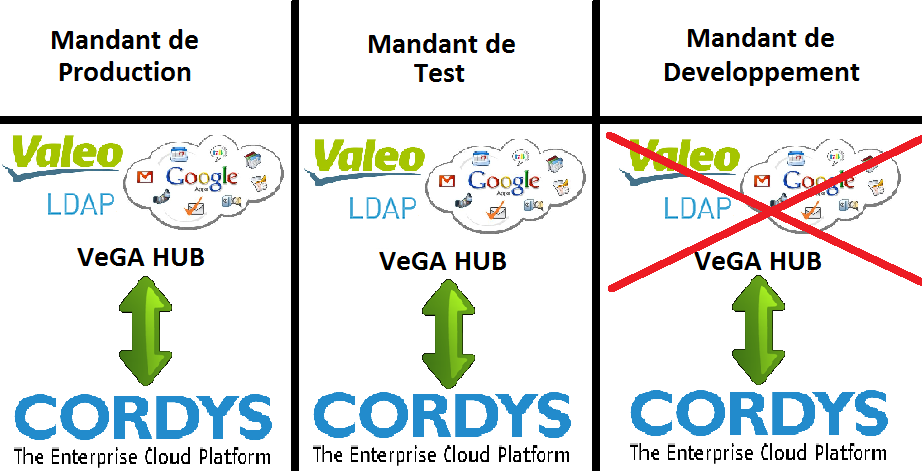
\includegraphics[height=9.25cm]{architecture_Cordys.png}
	\caption{\textit{Schéma de l'architecture Cordys chez Valeo}}\label{image.architectureCordys} 
\end{figure}

\clearpage

\subsection{Présentation de l'interface standard d'une application}


L'interface d'une application Cordys est relativement identique quelque soit l'application.\\
Ainsi, quel que soit l'application, deux onglets sont systématiquement disponibles : \textit{My Page \& Setup}.
Le nom de l'application se situe en haut à gauche, se qui constitue un bon repère visuel.\\
En plus de celà, un menu déroulant ``Change Application", permet d'afficher la liste entière des applications auxquelles vous avez le droit d'accéder.

 \begin{figure}[H]
    \centering
    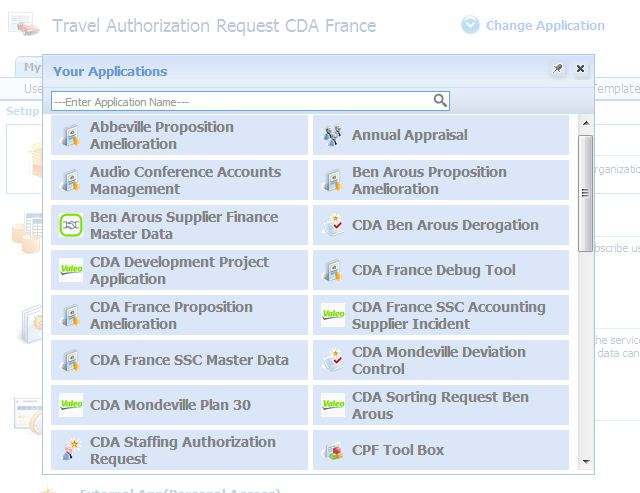
\includegraphics[height=6cm]{cordysChangeApplication.jpg}
	\caption{\textit{Interface Standard d'une application Cordys - Menu ``Change Application"}}\label{image.CordysChangeApplication} 
\end{figure}

\subsubsection{L'onglet My Page}

La vue par défaut d'une application est l'onglet: ``My Page". Il regroupe les dernières données relatives à l'utilisateur.

 \begin{figure}[H]
    \centering
    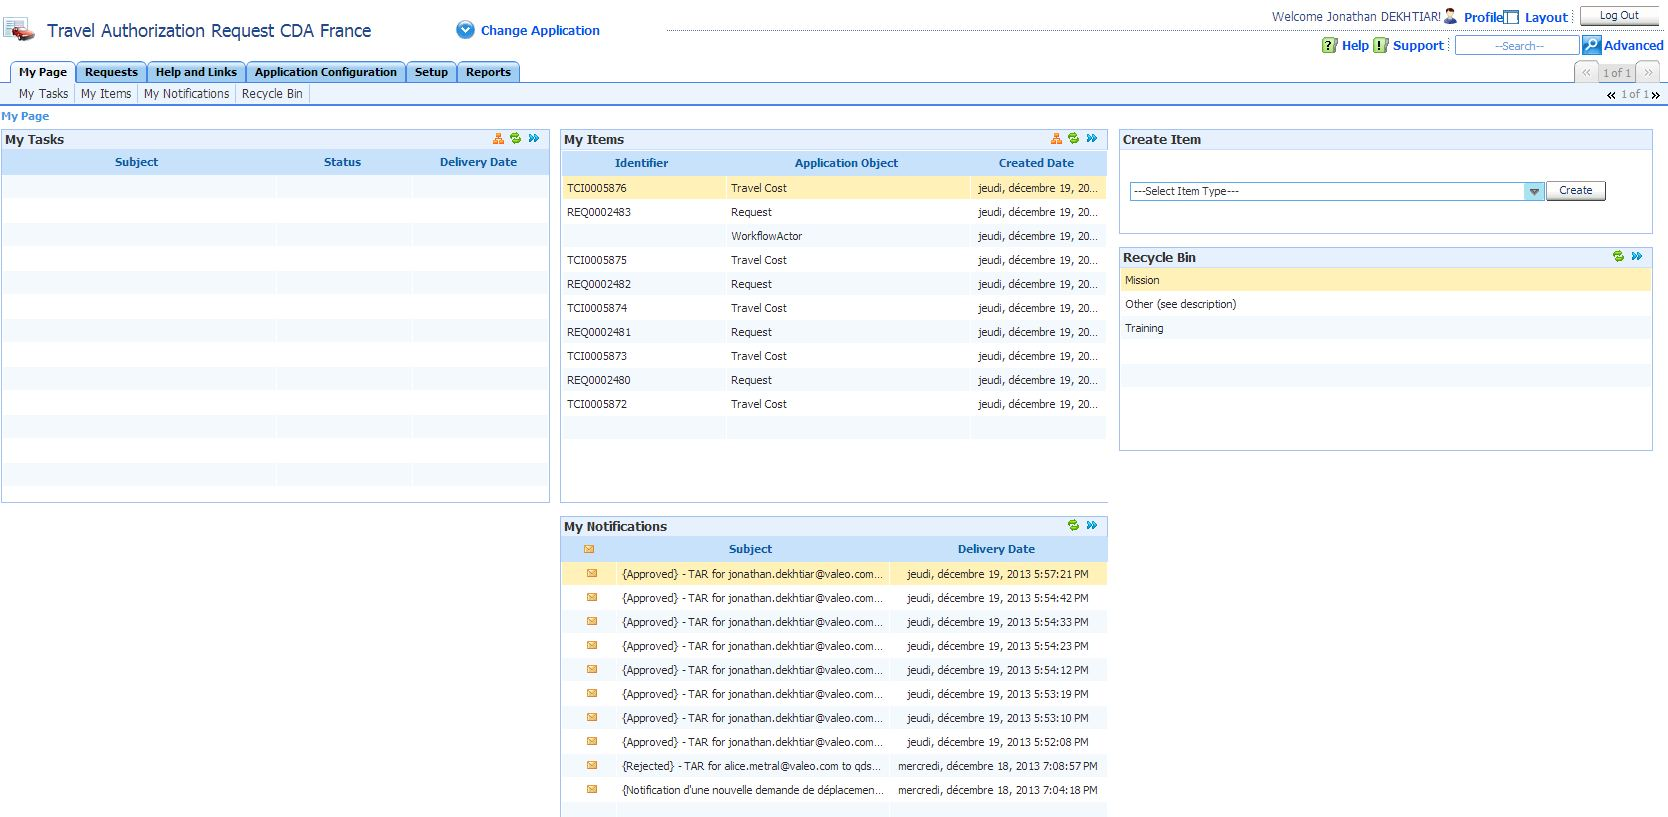
\includegraphics[height=8cm]{cordysMyPage.jpg}
	\caption{\textit{Interface Standard d'une application Cordys - Onglet ``My Page"}}\label{image.CordysMyPage} 
\end{figure}

\subsubsection{L'onglet Setup}

L'onglet Setup varie en fonction des droits d'accès. Un utilisateur aura accès uniquement à la personnalisation de son interface (de manière assez restreinte) et l'administrateur pourra, lui, accéder à plusieurs rubriques permettant l'import de données dans l'application, l'analyse des processus en cours d'éxécution, les tâches actuellement en attentes (et les réaffecter si nécessaire), la liste des utilisateurs de l'application et leurs droits respectifs (en lecture et en modification), ainsi que d'autres fonctions moins utiles comme les modèles d'emails ou l'état des nombres auto-incrémentés.

 \begin{figure}[H]
    \centering
    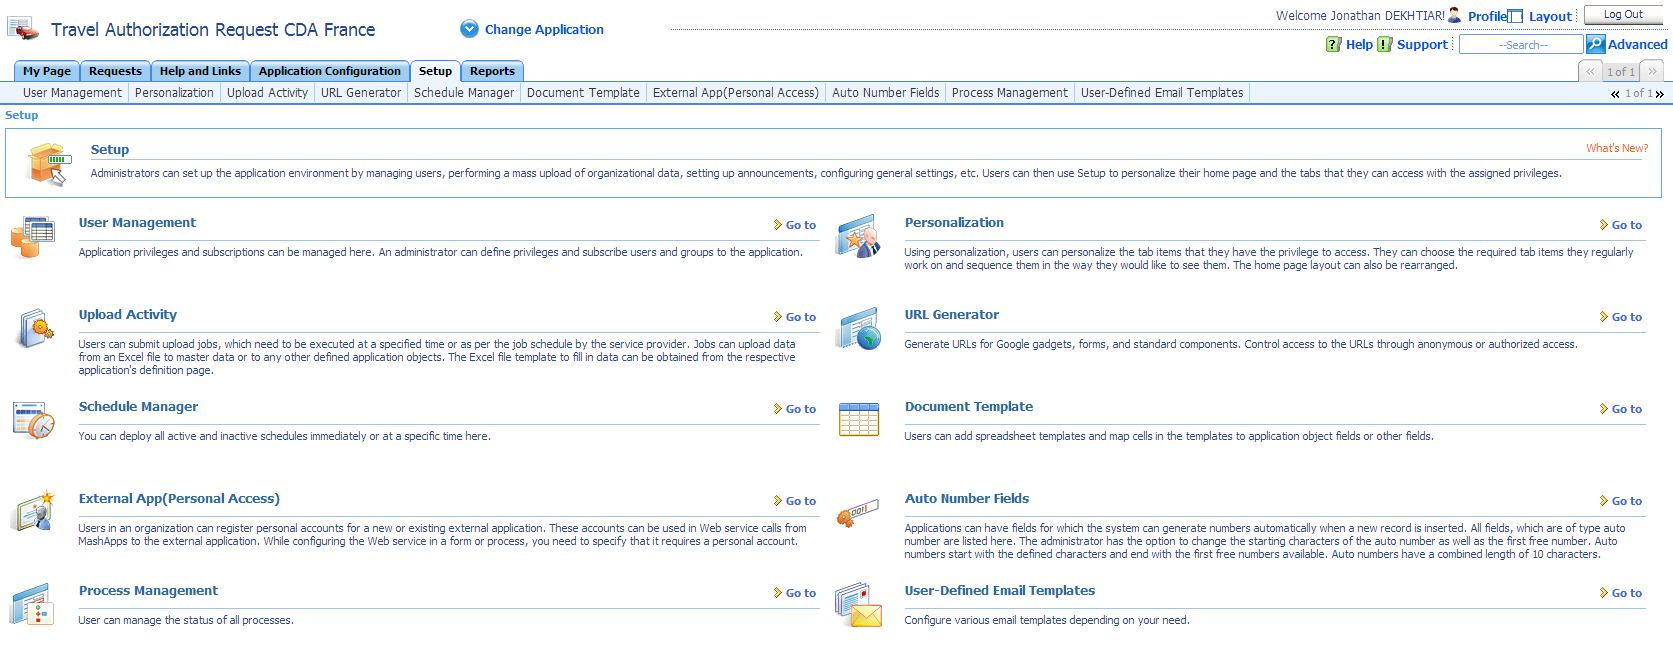
\includegraphics[height=7cm]{cordysSetupAdmin.jpg}
	\caption{\textit{Interface Standard d'une application Cordys - Onglet ``Setup" - Vue Administrateur}}\label{image.CordysSetupAdmin} 
\end{figure}

 \begin{figure}[H]
    \centering
    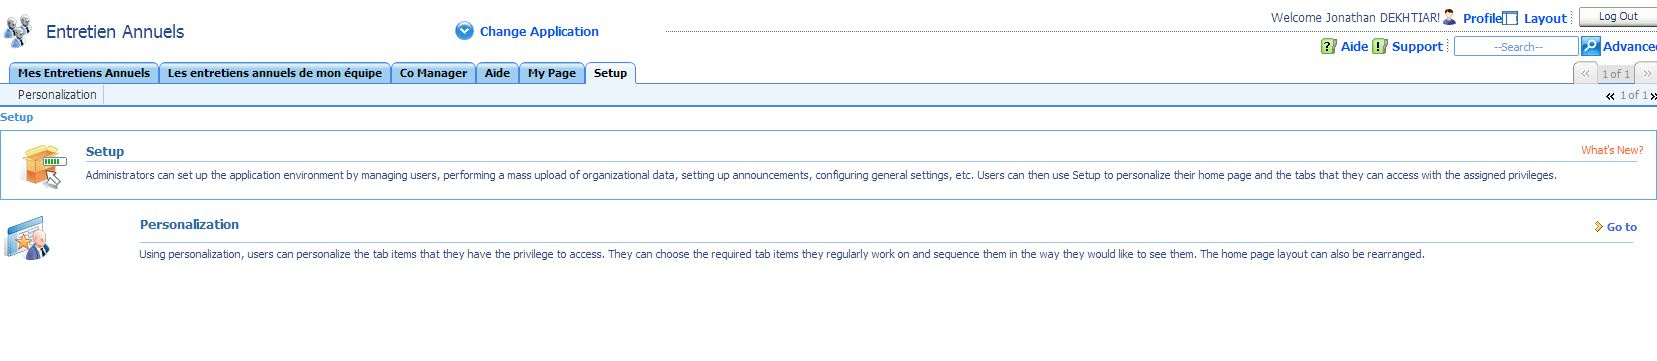
\includegraphics[height=3.8cm]{cordysSetupUser.jpg}
	\caption{\textit{Interface Standard d'une application Cordys - Onglet ``Setup" - Vue Utilisateur}}\label{image.CordysSetupUser} 
\end{figure}

\clearpage

\subsubsection{L'onglet Report}

L'onglet Report est automatiquement disponible pour chaque application, cependant l'administrateur peut choisir ou non de le faire apparaitre dans l'application et/ou de le rendre disponible uniquement pour une partie des utilisateurs ou pour tout le monde en modifiant les droits d'accès.

Les Reports sont à ``paramétrer" en développement pour qu'ils apparaissent en production de manière systématique. Sinon ``\emph{l'instant Report}" permet d'extraire des données de manière rapide et flexible. Il est cependant plus long à effectuer qu'un Report automatique et nécessite la connaissance du nom des champs que l'on veut extraire.

 \begin{figure}[H]
    \centering
    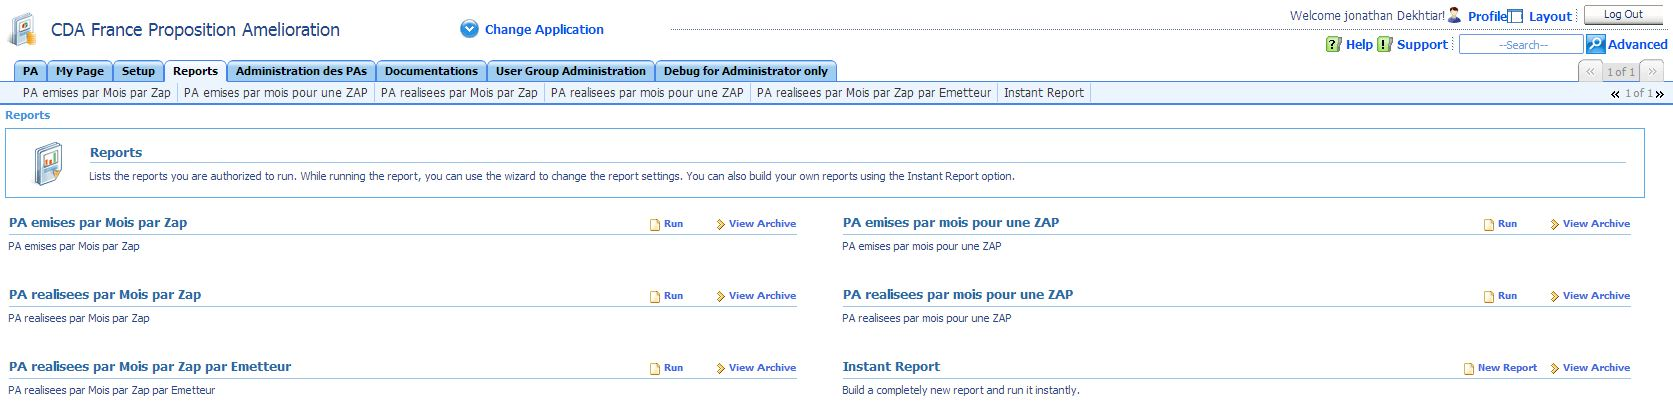
\includegraphics[height=3.8cm]{cordysReports.jpg}
	\caption{\textit{Interface Standard d'une application Cordys - Onglet ``Report"}}\label{image.CordysReports} 
\end{figure}

\clearpage

\subsection{Présentation de l'interface developpeur de Cordys}

\subsubsection{La page d'accueil de la plateforme de développement}

La page d'accueil de la plateforme de développement est assez sobre, on y retrouve les différentes sections sur la gauche et une vue ``graphique" au centre expliquant à quoi sert cet onglet. Toujours dans l'optique de permettre à un utilisateur, sans bagage informatique, de pouvoir mettre en place simplement et rapidement en place une application.

 \begin{figure}[H]
    \centering
    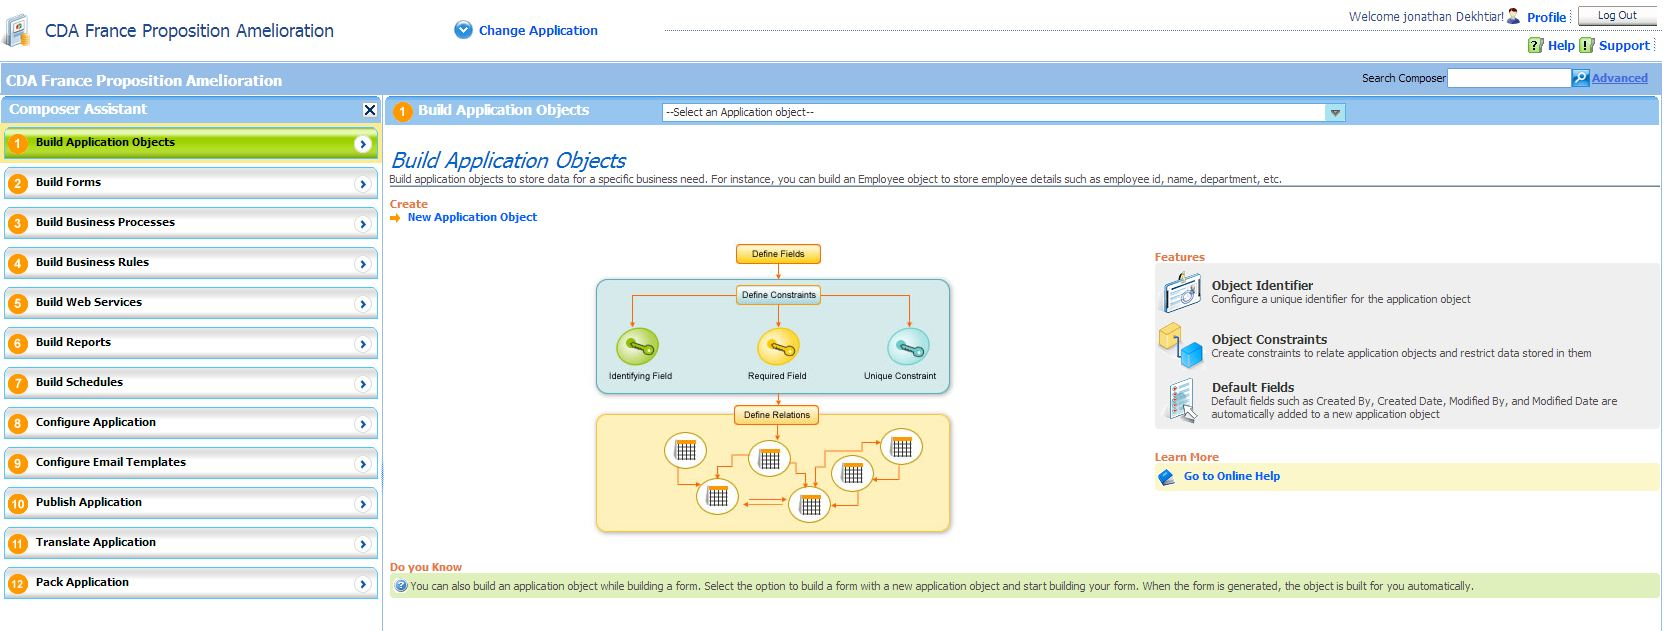
\includegraphics[height=6.9cm]{cordysDevHome.jpg}
	\caption{\textit{Interface de développement de Cordys - Page D'accueil}}\label{image.CordysDevHome} 
\end{figure}

\subsubsection{L'onglet ``Application Object"}

Un \emph{Application Object} est l'équivalent de ce qu'on appelle en programmation orientée objet : \textbf{un objet}.\\
Ces objets sont la base de l'application, ils sont à définir selon les besoins et donc selon le cahier des charges qui a été établi au préalable.\\
Des diagrammes UML sont donc à prévoir sur les applications lors de la définition du projet.

Les \emph{Application Objects} permettent de stocker les données relatives à l'entreprise. Par exemple, les dépenses de l'entreprise dans une application dédiée à la validation des factures ou au remboursement des frais des employés.

Afin de stocker des données dans un \emph{Application Object}, il est nécessaire d'ajouter donc des champs relatifs à l'utilisation (Exemple: FactureID, UserName, ApproverName, ...).

Lors de la création de l'\emph{Application Object}, il est possible de définir la clé primaire, des index afin de faciliter et accélerer la recherche et des contraintes (sur un ou plusieurs champs).

Tous les \emph{Application Object} sont stockés dans l' \emph{``Application Object Repository"}. Il est ainsi possible de les modifier, et de les supprimer par l'intermédiaire de ce répertoire.

 \begin{figure}[H]
    \centering
    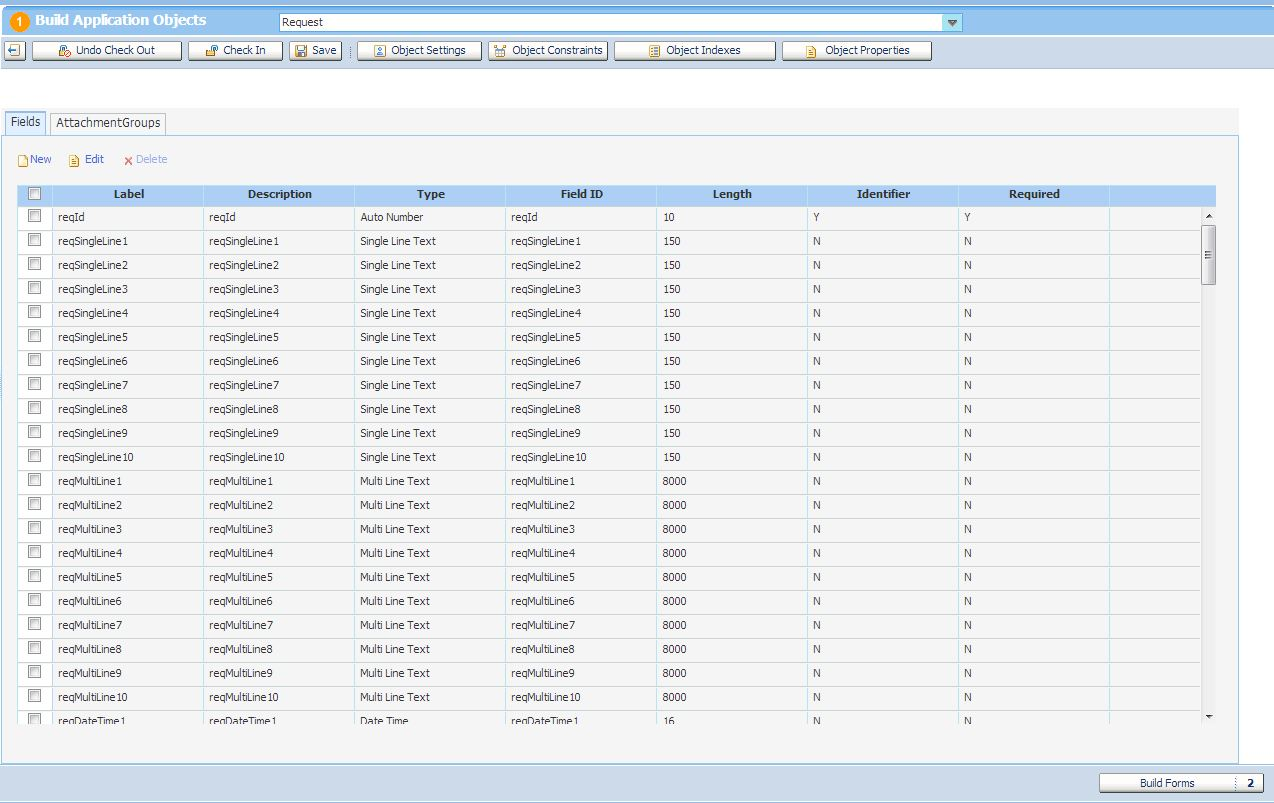
\includegraphics[height=11cm]{cordysDevAOForm.jpg}
	\caption{\textit{Interface de développement de Cordys - Interface de définition des Application Object}}\label{image.CordysDevAOForm} 
\end{figure}

\clearpage

\subsubsection{L'onglet ``Forms"}

Une fois un \emph{Application Object} défini, il est possible de créer un ou plusieurs formulaires de manière à permettre l'instanciation de ces objets. Tous les champs relatifs à cet \emph{Application Object} sont automatiquement ajoutés au formulaire, charge au développeur de choisir s'il désire tous les garder et de les agencer à sa convenance.\\
Il est également possible de créer un formulaire sans le rattacher à un \emph{Application Object}. Dans ce cas, il est impossible de sauvegarder les informations entrées dans ce formulaire et celles affichées par les différents Web-Services appelés.

Différents outils sont à disposition afin de mettre en place le formulaire répondant exactement aux attentes: 

\begin{itemize}\itemsep5pt
	\item \textbf{Les Types de Sections: }Il possible de créer différent types de section pour organiser les champs du formulaire. Ces sections portent le nom de : ``Group Box", ``Grid", et  ``Tab sections". Il est également possible de créer une section pour attacher un ou plusieurs fichiers et des éventuels commentaires.
		
	\item \textbf{Les types de Champs: }De nombreux types de champs sont à disposition des développeurs, le choix dépend alors du type d'information qui y sera stocké.
	
	\item \textbf{Le ``Repertoire" de Web Services: }Tous les Web services de l'application sont stockés dans un répertoire. Il est ainsi possible d'ajouter des Web Services, basés sur des Application Objects et Business Process, à un formulaire directement depuis ce répertoire. Il est également possible d'ajouter des Web Services ``externes" SOAP ou REST.
	
	\item \textbf{Les Paramètres de Formulaire: }Une des sources de flexibilité dans la création des formulaires vient de ce qu'on appel les ``Form Parameters" ou en Français : Les Paramètres de Formulaire. Ils permettent de définir quels champs seront les entrées ou les sorties d'un ou plusieurs Web Services.
	
	\item \textbf{Design adaptatif: }Les formulaires peuvent être créés de manière ``flexible" et s'adapter à la taille de la fenêtre ou du design établi (\textit{Responsive Design}). Les Sections, champs et Web Services peuvent être placés de manière quelconque dans le formulaire.
			
	\item \textbf{Les champs de type ``Lookup": }Il est possible de paramétrer des champs pour les associer à un ``\emph{lookup}". Cela leur permettra de \textbf{sélectionner} des données relatives à des Application Objects ou aux Utilisateurs (Groupes, Fonction, Email  ...).

	\item \textbf{Les règles de Formulaire: }Il est possible de définir des conditions qui vont modifier le comportement d'un formulaire en utilisant ce qu'on appelle une ``Règle de Formulaire". Il est ainsi possible d'assigner des valeurs, afficher des messages, cacher ou forcer l'affichage, bloquer ou débloquer un champs, une section.
	
	\item \textbf{Les vues: }Il est possible de créer des vues de manière à trier les données pour les formulaire de type tableau ou ``Grid" en anglais.
	
	\item \textbf{L'éditeur de Script: }Ce dernier module permet aux développeurs plus chevronnés d'avoir un contrôle total de leur formulaire avec l'aide du Javascript et un petite sur-couche \textit{made in Cordys}.

\end{itemize}

En dehors des fonctions citées plus haut, un système de versionnement est en place et permet d'afficher les dix dernières révisions de l'objet ou du formulaire via un système de ``Check In" / ``Check Out"  dans le but d'améliorer l'efficience et de réduire la maintenance. Il est également possible de modifier le formulaire de sauvegarder et de ne finalement rendre les modifications effectives que plusieurs jours après en effectuant le ``Check In" au bon moment.

Il est possible de prévisualiser le formulaire pendant son édition. Cette fonction permet de vérifier le bon comportement pendant l'exécution (en particulier les scripts et règles de formulaires).
\vspace{8mm}

\begin{figure}[H]
    \centering
    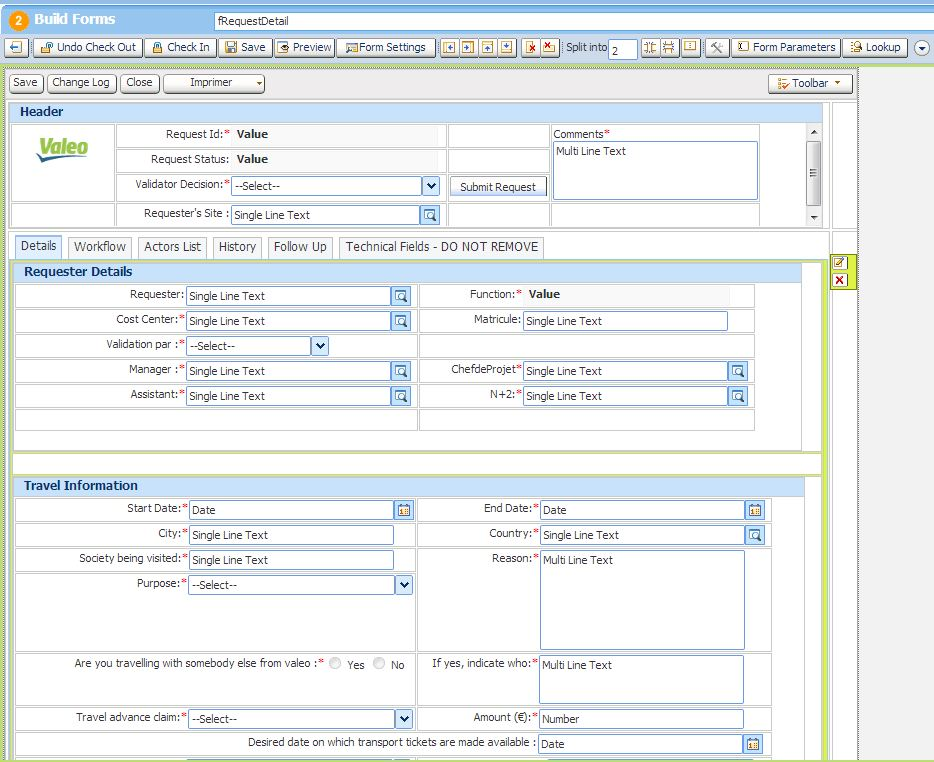
\includegraphics[height=14.5cm]{cordysDevFormsDef.jpg}
	\caption{\textit{Interface de développement de Cordys - Interface de définition des Formulaires}}\label{image.cordysDevFormsDef1} 
\end{figure}

\clearpage
\subsubsection{L'onglet ``Business Process"}

C'est la notion clé du système Cordys, et d'ailleurs mon sujet de stage mentionne cet élément sous le nom de \textbf{Workflow}. Ce n'est donc pas un outil à proprement parlé mais plutôt une finalité: sa mise en place.

Un Business Process est donc un ensemble d'activités liées qui produisent un service de manière à atteindre les objectif du business. Les ``Business Processes" sont \textbf{la manière} d'effectuer une tâche spécifique au sein d'une organisation spécifique. 
Un Business Process définit, dans notre cas, un parcours de validation ou signature et ainsi aide les employés à interagir avec les différentes entités de l'entreprise.



Pour exemple, prenons l'approbation du remboursement d'une note de frais :

Un employé peut avoir des dépenses durant un voyage d'affaire et doit être remboursé. Ainsi il serait intéressant d'établir un \textbf{Business Process} décrivant le parcours de signature à effectuer de manière à donner l'autorisation de manière automatique à la finance pour le paiement de la note de frais:\\
Demande de remboursement => Validation du supérieur hiérarchique => Validation du chef de projet => Demande de remboursement validée. \\
Il peut être judicieux de notifier tout le monde dès l'acceptation ou le refus de la demande. Le remboursement peut ainsi être débloqué par le service financier.

Automatiser ce genre de processus permet d'une part de limiter les erreurs humaines et d'autres part d'en maximiser l'efficience et la traçabilité.

Un Business Process se définit par:

\begin{itemize}\itemsep7pt

	\item \textbf{Un But: } Un Business Process possède un but bien défini, qui est le besoin Business d'une action systématique.
	
	\item \textbf{Des données en ``entrée": }Un Business Process a besoin de données en entrée, que l'on appelle ``ressources", pour fonctionnner. Pour exemple, reprenons notre exemple de la validation des notes de frais. Voici quelques ressources : Date du début du Voyage, Date de fin du voyage, montant de la note de frais, Utilisateur demandeur ...
	
	\item \textbf{Des données en ``sortie: "}Un Business Process produit une ou plusieurs sorties qui fournissent des informations importantes pour l'entreprise.
	
\end{itemize}

Il est possible de publier un Business Process et de l'intégrer à un formulaire à la manière d'un Web Service. Il est ensuite possible de définir les ``déclencheurs" qui vont appelés le Business Process à intervalle régulier ou sous certaines conditions.

\begin{figure}[H]
    \centering
    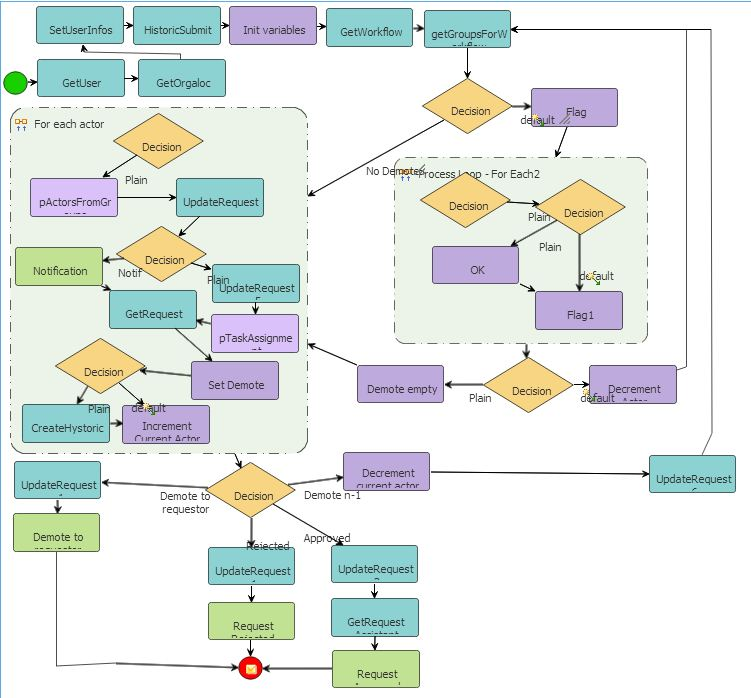
\includegraphics[height=17cm]{cordysDevBusinessProcess.jpg}
	\caption{\textit{Interface de développement de Cordys - Exemple d'un Business Process}}\label{image.cordysDevFormsDef2} 
\end{figure}
\clearpage

\subsubsection{L'onglet ``Business Rules"}

Les ``Règles Business" sont des collections de procédures qui commandent une organisation et les services qui lui sont rattachés. Ils définissent les contraintes qui s'appliquent et aident à suggérer les activités clés du Business Process au moment opportun. Ils préparent et présentent les données de manière à faciliter les prises de décision critiques et stratégiques. 

Une ``règle Business" peut appeller un Business Process, envoyer des notifications, ou afficher des avertissements. Par exemple, une règle Business peut orienter le choix d'un Business Process ou d'un autre en fonction du montant de la note de frais pour reprendre notre exemple. (Si le montant de la note de frais est supérieur à 1000€ => Demander la validation du Directeur d'usine). 

Pour résumer, une règle Business est un ensemble de conditions et d'actions. Structure algorithmique classique en \emph{IF-THEN } et multiples \emph{ELSE-IF}.


Voici le type d'actions que peut effectuer une ``règle Business" lorsqu'une de ses conditions d'exécution est vérifiée:

\begin{itemize}\itemsep7pt
	 \item \textbf{Assigner une valeur à un champs d'un formulaire ou d'un Application Object.}
	 	 
	 \item \textbf{Arrêter une transaction en cours et en notifier l'utilisateur par l'affichage d'un message.}
	 
	 \item \textbf{Envoyer une notification à un utilisateur.}
	 
	 \item \textbf{Déclencher un Business Process.} 
\end{itemize}

\subsubsection{L'onglet ``Web Services"}

Un Web Service  est une fonction logicielle construite pour réaliser des interactions machine à machine par l'intermédiaire d'un réseau. Ils utilisent un modèle standardisé de données comme: XML / SOAP / WSDL. XML est utilisé pour le formatage des données, SOAP pour effectuer le transfert des données, et WSDL pour décrire le service.

Les Web Services permettent une communication entre plusieurs applications originaires de différentes sources, le tout avec un temps de réponse au plus court et une compatibilité multi-plateforme grâce au formatage XML des données.\\
Ainsi une application en Java peut communiquer avec une application en Perl fonctionnant sur Unix ou Windows.

Cordys permet une génération automatique d'une série de Web Services Standards pour chaque Application Object : Lecture, Ecriture, Modification, Suppression.\\
Il est également possible de construire des Web Services plus avancés grâce à l'assistant dédié.

\clearpage

\subsubsection{L'onglet ``Configure Application"}

Après la création et le paramétrage de tous les éléments de l'application, il devient nécessaire de configurer l'application et ses différents onglets.

Ces onglets peuvent regrouper un ou plusieurs formulaires et chaque formulaire et/ou onglet peut être accessible ou non en fonction du privilège utilisateur.

Les privilèges utilisateurs sont à créer et à modifier dans cette section. Seul le droit administrateur est automatiquement en place, il permet un accès total à l'application.

Il est également possible de référencer une application comme source, cette dernière sera accessible à travers l'application actuelle (en particulier lors des Look-Ups)

\subsubsection{Creation d'un ``\emph{Application Package}"}

Une fois l'application prête pour être testée dans le mandant de test, il est nécessaire de générer un "Application Package" soit dans le but de créer une sauvegarde de l'application à l'instant T soit pour la déployer dans un autre mandant.
\clearpage

\section{Titre de Fonction : ``Automation Analyst"}

\subsection{Description de mon rôle}

Mon rôle a été principalement orienté sur deux objectifs. En effet il m'a été demandé d'une part, de développer des améliorations sur un parc applicatif existant (en particulier par rapport aux attentes des ``Business Owners") ainsi que de développer et de déployer de nouvelles applications, d'autres part, il m'a été demandé d'effectuer le support applicatif sur ces mêmes applications via un système open source de tickets: GLPI.\\
Finalement, il m'a été demandé d'effectuer des formations \emph{orientées utilisateur} sur plusieurs sites Français à propos de l'utilisation des applications déployées en production.

Ce genre de poste demande donc une double compétence:

\begin{itemize}\itemsep7pt

	\item En effet, il nécessaire de connaître parfaitement son outil et la plateforme afin de développer la fonction qui manque ou d'améliorer l'interface d'une application. Une faculté d'analyse et d'adaptation rapide sont donc les qualités humaines prépondérantes dans cette activité en plus des connaissances techniques.
	
	\item Le deuxième rôle est d'effectuer un support relatif à une quinzaine d'applications. Il est donc extrêmement courant de d'interagir avec tout type d'utilisateur et ce plusieurs fois par jour. Le problème réside dans le fait que l'on ne connait que rarement son interlocuteur, tout comme sa fonction dans l'entreprise. Il faut donc être capable d'adapter son discours en fonction des connaissances de l'utilisateur, de son ``empressement" et de sa fonction dans l'entreprise. Il est donc critique d'avoir de bonnes facultés de communication (en anglais et français), une certaine capacité de discernement et de répartie.
	
\end{itemize} 

\clearpage

\subsection{Retour sur expérience}

\subsubsection{La partie technique}

Concernant la partie technique, Cordys Process Factory est très peu documenté. Impossible de trouver un manuel ou même une documentation officielle. Valeo possède ses propres modules de formation mais cela reste très succinct et ce fût très complexe de me former à  son utilisation, l'administration de la plateforme et particulièrement au développement sur cette plateforme. Malgré une formation intensive de deux jours à Paris, autonomie et des dizaines d'heures à tâtonner sur la plateforme furent les maitres mots de mon expérience sur Cordys Process Factory.

Un Forum Valeo pour les développeurs sur Cordys est en place, cet outil me fut d'un grand secours, surtout durant les premiers mois de mon stage.
Malgré cela je ne pense toujours pas maitriser la plateforme. Je connais les fonctions et les éléments qui me permettent de faire ce dont j'ai besoin, mais sur une demande trop spécifique ou trop pointue il m'est nécessaire de demander de l'aide. Cordys est une plateforme propriétaire de \textbf{développement au clic}, très peu de code est à mettre en place. Ce qui signifie que si vous ne savez pas où cliquer pour effectuer telle ou telle action, vous pouvez chercher pendant des heures avant que la solution vous apparaisse. A l'inverse d'un langage de programmation qui, pour la plupart, malgré ses spécificités, reste similaire à de nombreux autres et avec de solides connaissances en algorithmique et une documentation il est relativement aisé d'arriver à ses fins.

\subsubsection{La partie communicationnelle}

C'est sans aucun doute la partie qui m'a demandé le plus d'efforts. Tant dans la forme que dans le fond. En effet, je m'étais majoritairement adressé, auparavant, à des personnes connaissant l'informatique dans le cadre de mes études. Et ce ne fut pas forcément aisé d'adapter mon discours aux connaissances de mon interlocuteur et surtout au fait que je ne sache jamais à qui je m'adresse. Un environnement comme celui de Valeo est très complexe et demande de grandes précautions lorsque l'on s'adresse à quelqu'un. Il est donc primordial d'\textbf{apprendre} à ne s'engager sur quelque chose même si on le croit acquis et 100\% sûr. En effet, ce qui est possible dans un environnement quelconque n'est pas forcément possible dans l'environnement Valeo. A la fois d'un point de vue technique et également parce que l'on ne maitrise pas tous leviers d'une action et qu'il faut obtenir l'accord d'un certains nombre de personnes avant de pouvoir déclencher certaines actions.

J'ai personnellement eu beaucoup de mal à gérer la pression durant les deux premiers mois. En effet, un environnement comme Valeo demande que tout soit fait en flux tendu et en parallèle voir limite ``pour hier" pour ne paraphraser personne. C'est une situation à laquelle je n'avais jamais fait face, il a fallu \textbf{apprendre} à ne pas paniquer et se recentrer sur l'objectif, définir des priorités, gérer les timings et le tout de manière relativement automatique et intuitive car il n'est pas envisageable de passer plusieurs heures par semaine à établir un diagramme de Gantt pour la semaine. La \emph{liste des tâches} à effectuer de Google fut sans aucun doute mon meilleur allié pendant ce stage.
